\section{Summary, Conclusion and Future Work}
\subsection{Summary}
\begin{frame}
\frametitle {Summary and Conclusion of work done}
\begin {center}
\begin{itemize}
\item NoC has been used as a data routing medium, which takes care of routing congestion
\item NoC partitioning will help isolating application node from the communication infrastructure
\item NoC integration with High speed serial Aurora Core very useful for Multi FPGA implementation
\item Quasi-SERDES module between routers of partitioned NoC is a viable alternate
\item Automation of NoC partitioning with inter-chip communication link integration using python scripts reduces the manual work tremendously
\end {itemize}
\end{center}
\end {frame}


\begin {frame}
\frametitle {Summary and Conclusion of work done (contd.)}
\begin {center}
\begin {itemize}
\item LDPC has a complex interconnect network, partitioned NoC can be used for data routing in Multi FPGA implementation
\item Bezier interpolation tested using DE0-Nano and Raspberry Pi working at 50 MHz converges in 0.161 seconds
\item Raspberry Pi can be used as FPGA/CPLD JTAG configuration (tested) and debugging platform (not tested)
\item FPGA/CPLD (Krypton board designed at WEL lab) can be configured using Raspberry Pi (tested), this is a suitable choice for remote lab set-up
\item Raspberry Pi interfacing with FPGA presents a viable software hardware co-design platform
\end {itemize}
\end{center}

\normalsize
\end {frame}

\subsection{Future Work}
\begin{frame}
\frametitle {Future Work}
\begin {center}
\begin {itemize}
\item Design of a scalable and a repeatable block style design of FPGA PCB for Multi-FPGA NoC implementation
\item A simple PCB design shown below which could be repeated to create n$\times$n Mesh of FPGA Network-of-Chips shown in the next slide
\end {itemize}
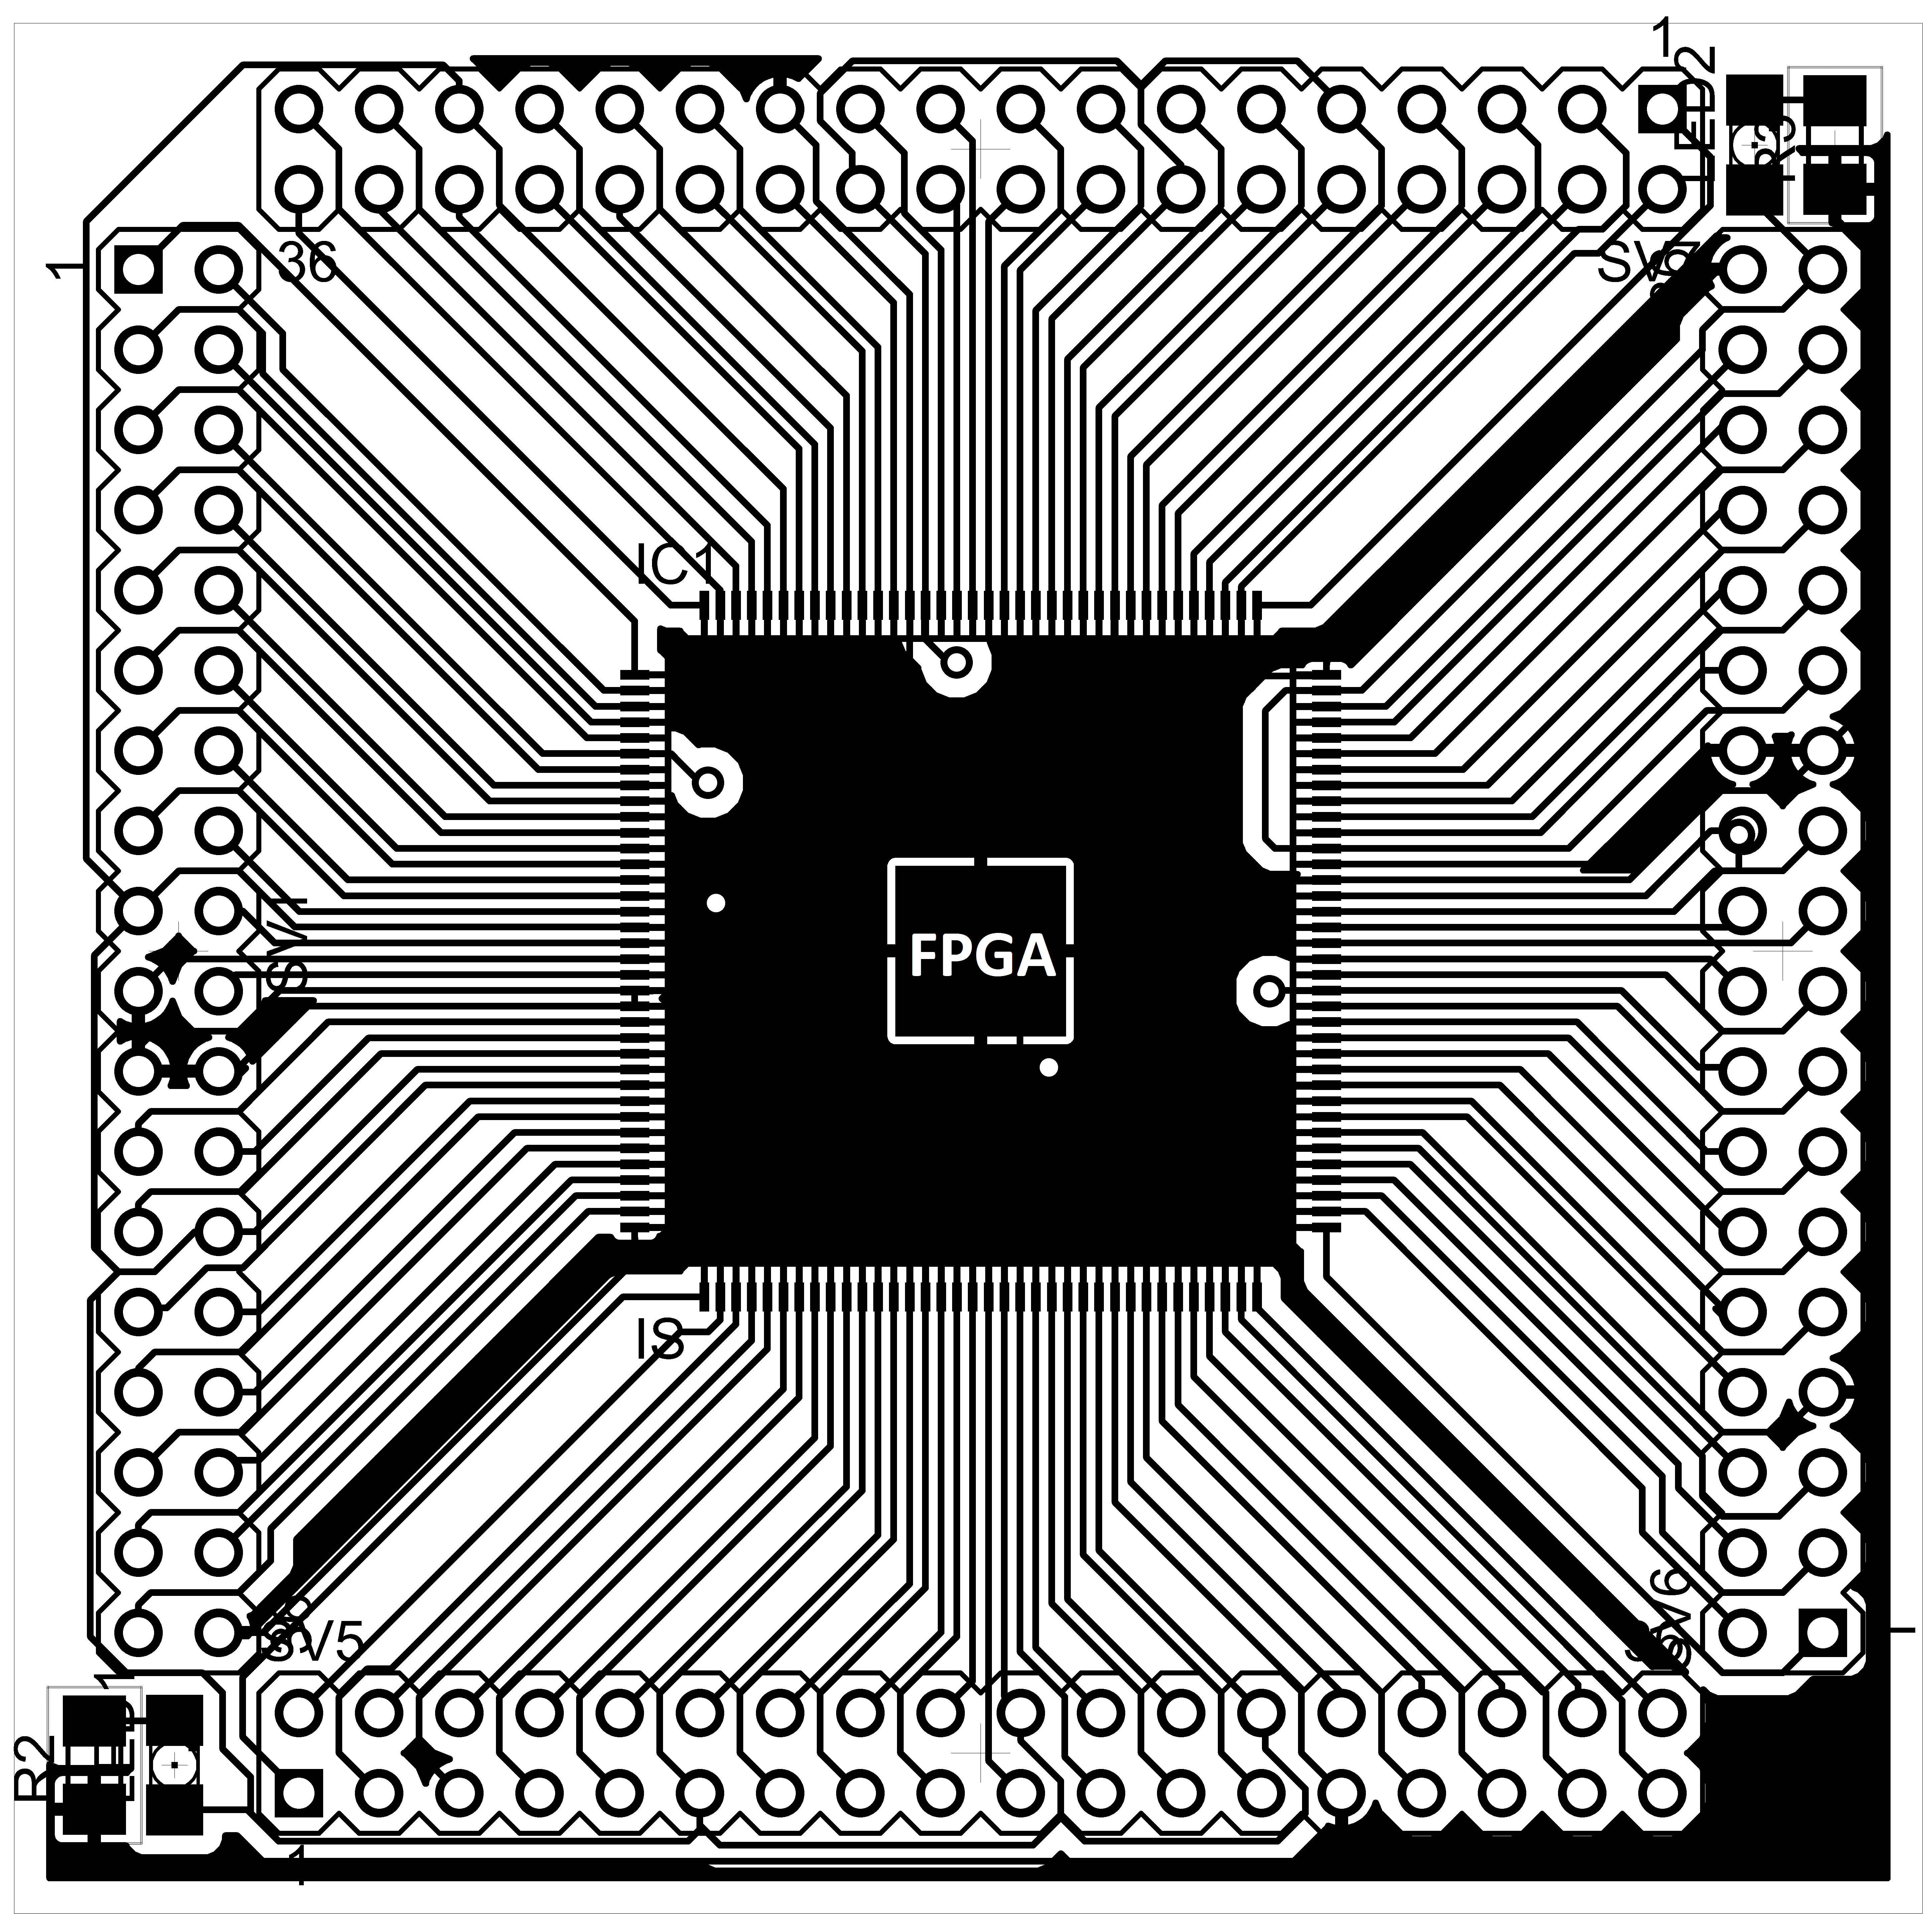
\includegraphics[scale=0.5]{./figs/BasicPCB}
\end {center}
\end{frame}

\begin{frame}
\begin {center}
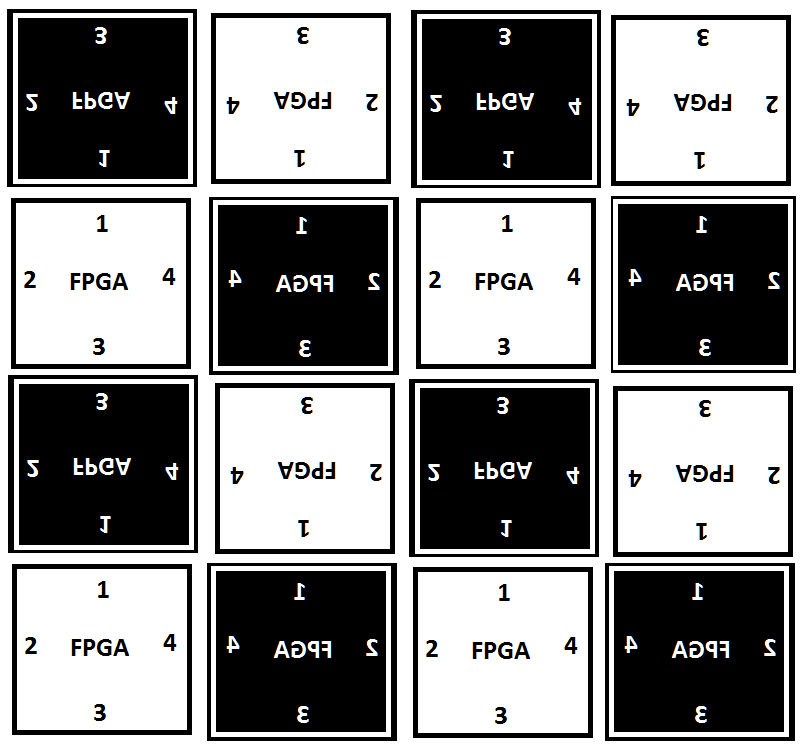
\includegraphics[scale=0.3]{./figs/MultiFPGANoC}
\end {center}
\end{frame}

\subsection{References}

\begin{frame}
\frametitle{Reference}
\begin{thebibliography}{10} 
\small
\bibitem {yatish_ddp} Yatish Turakhiya
``Multi-FPGA Hardware Acceleration of Boolean Matrix Vector Multiplication using Network-on-Chip``,
\emph{DDP Thesis- Dept. of Electrical Engineering, IIT Bombay}

\bibitem {Shaishav_mtp} Shaishav Shah, 
``LDPC Decoder Implementation using NoC``,
\emph{EEE Transactions on Information Theory, pages 2711–2736, 2001}

\bibitem {connect_noc} Michael K. Papamichael, 
``Fast Scalable FPGA-Based Network-on-Chip Simulation Models``
\emph{Computer Science Department, Carnegie Mellon University}


\end{thebibliography}
\end{frame}

\begin{frame}
\frametitle{Reference}
\begin{thebibliography}{10} 
\small
\bibitem {tanner_graph_journaltanner_graph_journal} Tanner, Robert Michael
\emph  {EA recursive approach to low complexity codes. }

\bibitem {five} Kouadri-Mostefaoui, A.-M. and Senouci, B. and Petrot, F., 
``Scalable Multi-FPGA Platform for Networks-On-Chip Emulation``,
\emph{Technical Report- Dept of Electrical Engineering, IIT Bombay}

\bibitem {fourteen} Kumar, S. and Jantsch, A. and Soininen, J.-P. and Forsell, M. and Millberg, M. and Oberg, J. and Tiensyrja, K. and Hemani, A.
\emph  {A network on chip architecture and design methodology. }

\bibitem {935594} Dally, W.J. and Towles, B.
``Design Automation Conference, 2001. Proceedings``,
\emph{PhD thesis, IIT Bombay, India, 2012}

\end{thebibliography}
\end{frame}


\begin{frame}
\begin{center}
Thank You 
\end{center}

\end{frame}

